\chapter{Harmony of Numbers}

\begin{quote}
%Nature uses as little as possible of anything.  

Let us despise the barbaric neighings [of war] which echo through
these noble lands, and awaken our understanding and longing for the
harmonies.

\hfill---Johannes Kepler
\end{quote}

\begin{teachingnote}
This section is a hodge-podge of applications and modeling.
\end{teachingnote}

\begin{activitynote}
Activity~\ref{A:orderMod} complements this section well.
\end{activitynote}

\section{Clocks}

It is now time to think about clocks. Consider the usual run-of-the-mill clock:
\[
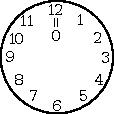
\includegraphics{../graphics/clock.pdf}
\]
\begin{question}
Suppose you start grading papers at $3$ o'clock and then $5$ hours
pass. What time is it? Now suppose that you find more papers to grade,
and $5$ more hours pass---now what time is it? How do you do these
problems? Why are there so many papers to grade?
\end{question}
\QM

We have a mathematical way of writing these questions:
\begin{align*}
3 + 5 &\equiv 8 \pmod{12} \\
8 + 5 &\equiv 1 \pmod{12} 
\end{align*}
We call arithmetic on clocks \textbf{modular arithmetic}.
\index{modular arithmetic} Being rather fearless in our quest for
knowledge, we aren't content to stick with $12$ hour clocks:
\[
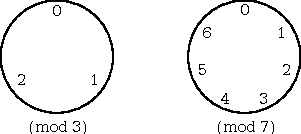
\includegraphics{../graphics/moreclocks.pdf}
\]

\begin{question}
Suppose you are working on a $2$ hour clock:
\[
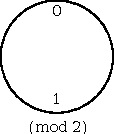
\includegraphics{../graphics/twoclock.pdf}
\]
Suppose you started at time zero, and finished after 10245
hours. 
\begin{enumerate}
\item Where is the hand of the clock pointing? 
\item How does the answer change if you are working on a $5$ hour
  clock?
\item What if you are working on a $7$ hour clock?
\end{enumerate}
\end{question}
\QM




OK---clocks are great. Here is something slightly different: Denote
the set of all integers that are $r$ greater than a multiple of $5$ by
$[r]_5$. So for example:
\[
[0]_5 = \{\dots,-15,-10,-5,0,5,10,15,\dots\}
\]
Write down the following sets:
\begin{align*}
[1]_5 &=  \raisebox{-3mm}{\fbox{\rule[0mm]{0mm}{7mm}\hspace{50ex}}} \\
[2]_5 &=  \raisebox{-3mm}{\fbox{\rule[0mm]{0mm}{7mm}\hspace{50ex}}} \\
[3]_5 &=  \raisebox{-3mm}{\fbox{\rule[0mm]{0mm}{7mm}\hspace{50ex}}} \\
[4]_5 &=  \raisebox{-3mm}{\fbox{\rule[0mm]{0mm}{7mm}\hspace{50ex}}} \\
[5]_5 &=  \raisebox{-3mm}{\fbox{\rule[0mm]{0mm}{7mm}\hspace{50ex}}} 
\end{align*}

\begin{question} With our work above, see if you can answer the following:
\begin{enumerate}
\item Explain why one could say that $[4]_5 = [9]_5$.
\item Explain why one could say that $[2]_5 = [-3]_5$.
\item Explain what you think is meant by the expression:
\[
[1]_5 + [2]_5 = [3]_5
\]
\item Explain what you think is meant by the expression:
\[
[1]_5 + [4]_5 = [0]_5
\]
\end{enumerate}
\end{question}
\QM



\begin{question}
How many different descriptions of modular arithmetic can you give? To aid you in this quest, I suggest you start your descriptions off with the words:
\begin{quote}
The number $a$ is congruent to $b$ modulo $m$ when \dots
\end{quote}
\end{question}
\QM

OK---I know I was supposed to leave that question for you, but there
is one description that I just gotta tell you about---check this out:
\[
a \equiv b \pmod{m} \qquad \Leftrightarrow \qquad a - b = m\cdot q
\]

\begin{question} 
What is the deal with the junk above? What is $q$? How does it help
you solve congruences like
\[
3x \equiv 1 \pmod{11}?
\]
\end{question}
\QM

\begin{question}
Is it the case that 
\[
5+x \equiv 2 + x \pmod{3}
\]
for all integers $x$? Why or why not? Use each of the descriptions
of modular arithmetic above to answer this question.
\end{question}
\QM







\newpage

\begin{problems}
\begin{enumerate}
\item Solve the following equations/congruences, expressing your
  answer as a number between $0$ and the relevant modulus:
\begin{enumerate}
\item $3 + x = 10$
\item $3 + x \equiv 10 \pmod{12}$
\item $3 + x \equiv 10 \pmod{7}$
\item $3 + x \equiv 10 \pmod{6}$
\item $3 + x \equiv 10 \pmod{5}$
\item $3 + x \equiv 10 \pmod{3}$
\item $3 + x \equiv 10 \pmod{2}$
\end{enumerate}
In each case explain your reasoning.
\item Solve the following equations/congruences, expressing your
  answer as a number between $0$ and the relevant modulus:
\begin{enumerate}
\item $10 + x = 1$
\item $10 + x \equiv 1 \pmod{12}$
\item $10 + x \equiv 1 \pmod{11}$
\item $10 + x \equiv 1 \pmod{9}$
\item $10 + x \equiv 1 \pmod{5}$
\item $10 + x \equiv 1 \pmod{3}$
\item $10 + x \equiv 1 \pmod{2}$
\end{enumerate}
In each case explain your reasoning.
\item Solve the following equations/congruences, expressing your
  answer as a number between $0$ and the relevant modulus:
\begin{enumerate}
\item $217 + x = 1022$
\item $217 + x \equiv 1022 \pmod{100}$
\item $217 + x \equiv 1022 \pmod{20}$
\item $217 + x \equiv 1022 \pmod{12}$
\item $217 + x \equiv 1022 \pmod{5}$
\item $217 + x \equiv 1022 \pmod{3}$
\item $217 + x \equiv 1022 \pmod{2}$
\end{enumerate}
In each case explain your reasoning.
\item Solve the following equations/congruences, expressing your
  answer as a number between $0$ and the relevant modulus:
\begin{enumerate}
\item $11+x \equiv 7 \pmod{2}$
\item $11+x \equiv 7 \pmod{3}$
\item $11+x \equiv 7 \pmod{5}$
\item $11+x \equiv 7 \pmod{8}$
\item $11+x \equiv 7 \pmod{10}$
\end{enumerate}
In each case explain your reasoning.

\item List out $6$ elements of $[3]_4$, including 3 positive and 3
  negative elements. Explain your reasoning.
\item List out $6$ elements of $[6]_7$, including 3 positive and 3
  negative elements. Explain your reasoning.
\item List out $6$ elements of $[7]_6$, including 3 positive and 3
  negative elements. Explain your reasoning.

\item One day you walk into a mathematics classroom and you see the
  following written on the board:
\begin{align*}
[4]_6 &=\{\dots, -14,-8,-2,4,10,16,22,\dots\}\\
\left[\frac{1}{2}\right] &=\left\{\dots, \frac{-3}{-6}, \frac{-2}{-4},
\frac{-1}{-2}, \frac{1}{2}, \frac{2}{4},\frac{3}{6},\dots\right\} 
\end{align*}
What is going on here? Can you figure out what $\left[\dfrac{3}{4}\right]$ would
be? Explain your reasoning.

\item If possible, solve the following equations/congruences,
  expressing your answer as a number between $0$ and the relevant
  modulus:
\begin{enumerate}
\item $3x = 1$
\item $3x \equiv 1 \pmod{11}$
\item $3x \equiv 1 \pmod{9}$
\item $3x \equiv 1 \pmod{8}$
\item $3x \equiv 1 \pmod{7}$
\item $3x \equiv 1 \pmod{3}$
\item $3x \equiv 1 \pmod{2}$
\end{enumerate}
In each case explain your reasoning.
\item Solve the following congruences, expressing your answer as a
  number between $0$ and the relevant modulus:
\begin{enumerate}
\item $11x \equiv 7 \pmod{2}$
\item $11x \equiv 7 \pmod{3}$
\item $11x \equiv 7 \pmod{5}$
\item $11x \equiv 7 \pmod{8}$
\item $11x \equiv 7 \pmod{10}$
\end{enumerate}
In each case explain your reasoning.
\item Solve the following congruences or explain why there is no
  solution, expressing your answer as a number between $0$ and the
  relevant modulus:
\begin{enumerate}
\item $15x \equiv 7 \pmod{2}$
\item $15x \equiv 7 \pmod{3}$
\item $15x \equiv 7 \pmod{5}$
\item $15x \equiv 7 \pmod{9}$
\item $15x \equiv 7 \pmod{10}$
\end{enumerate}
In each case explain your reasoning.
\item Make an ``addition table'' for arithmetic modulo $6$.
\item Make an ``addition table'' for arithmetic modulo $7$.
\item Make a ``multiplication table'' for arithmetic modulo $6$.
\item Make a ``multiplication table'' for arithmetic modulo $7$.

\item Explain the connection between writing an integer in base $b$ and
  reducing an integer modulo $b$.

\item Is 
\[
5 + x \equiv 12 + x \pmod{3}
\]
ever/always true? Explain your reasoning.
\item Is 
\[
20 + x \equiv 32 + x \pmod{3}
\]
ever/always true? Explain your reasoning.

\item Recalling that $i^2 = -1$, can you find ``$i$'' in the
  integers modulo $5$?  Explain your reasoning.
\item Recalling that $i^2 = -1$, can you find ``$i$'' in the
  integers modulo $17$?
  Explain your reasoning.
\item Recalling that $i^2 = -1$, can you find ``$i$'' in the
  integers modulo $13$?
  Explain your reasoning.
\item Recalling that $i^2 = -1$, can you find ``$i$'' in the
  integers modulo $11$?  Explain your reasoning.


\item Today is Saturday. What day will it be in 3281 days? Explain
  your reasoning.
\item It is now December. What month will it be in 219 months? What
  about 111 months ago? Explain your reasoning.
\item What is the remainder when $2^{999}$ is divided by $3$? Explain
  your reasoning.
\item What is the remainder when $3^{26}$ is divided by $7$? Explain
  your reasoning.
\item What is the remainder when $14^{30}$ is divided by $11$? Explain
  your reasoning.
\item What is the remainder when $5^{28}$ is divided by $11$? Explain
  your reasoning.
\item What is the units digit of $123^{456}$? Explain your reasoning.

\item Factor $x^2 + 1$ over the integers modulo $2$. Explain your
  reasoning.
\item Factor $x^3 +x^2 +x+1$ over the integers modulo $2$. Explain your
  reasoning.
\item Factor $x^5 +x^4 +x+1$ over the integers modulo $2$. Explain your
  reasoning.

\end{enumerate}
\end{problems}






\section{In the Real World}

Perhaps the coolest thing about mathematics is that you can actually
solve ``real world'' problems. Let's stroll through some of these
``real world'' problems.

\subsection{Automotive Repair}

\paragraph{A Geometry Problem}

One Thanksgiving Day I had a neat conversation with my cousin Chris at
the dinner table. You see he works on cars---specifically vintage
Italian sports cars. He had been doing some routine maintenance on one
of his cars and needed to remove the steering wheel and the steering
column.  All was fine until it came time to put the parts back
together. The steering wheel was no longer centered! The car could
drive down the street just fine, but when the car drove straight ahead
the steering wheel was off by a rotation of 5 degrees to the
right. This would not do!  This sounds like a geometry problem.


\paragraph{An Algebra Problem}

How did this happen you ask?  Well the
\index{steering!wheel}\textit{steering wheel} attaches to the car via
the \index{steering!column}\textit{steering column}:
\[
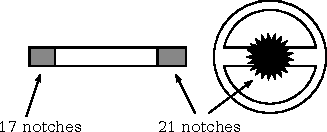
\includegraphics{../graphics/wheelcolumn.pdf}
\]
there were $21$ notches on the back of the wheel, which connects to
the column. There were also $17$ notches on the other end of the
column that then connected to the car itself.

Chris had noticed that moving the wheel 1 notch changed its position by 
\[
\frac{360}{21} \approx 17 \text{ degrees,}
\]
and that adjusting the columns by 1 notch changed its position by 
\[
\frac{360}{17} \approx 21 \text{ degrees.}
\]
Hmmm so if we want to center the wheel, we want to solve the following equation:
\[
17 w + 21 c = -5
\]
where $w$ represents how many notches we turn the wheel and $c$
represents how many notches we turn the column. Ah! This sounds like
an algebra problem! There is only one issue: We have two unknowns and
a single variable.


\begin{question}
How do we proceed from here? Can you solve the problem? Where does
modular arithmetic factor in to the solution?
\end{question}
\QM


\subsection{Check Digits}

Our world is full of numbers. Sometimes if you are in a large
organization---say a large university---you feel a bit like a
number. How do you know if you are the right number? Allow me to
clarify. Most items you buy have some sort of \index{UPC} UPC
(Universal Product Code) on them. This allows them to be put into a
computer in an organized fashion. When you buy items in a grocery
story, you want the item you scanned to come up---and not some other
(potentially embarrassing!) item. To ensure you get what is coming to
you, we have \index{check digits}\textit{check digits}. These are
digits that ``check'' to make sure that the code has scanned
correctly. Typically, what you see are either UPC-A codes or UPC-E
codes. Here is an example of a UPC-A code:
\[
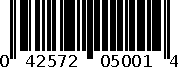
\includegraphics{../graphics/upcaEg.pdf}
\]
The check digit is the right most digit (in this case $4$). The check
digit is not used in identifying the item, instead it is used purely
to check if the other digits are correct. Here is how you check to see
if a UPC-A code is valid:
\begin{enumerate}
\item Working modulo $10$, add the digits in the odd positions and
  multiply by $3$:
\begin{align*}
0+2+7+0+0+1 &= 10\\
10\cdot 3 &= 30 \\
30 &\equiv 0 \pmod{10}.
\end{align*}
\item Working modulo $10$, add the digits in the even positions
  (including the check digit):
\begin{align*}
4+5+2+5+0 +4 &= 20 \\
20 &\equiv 0 \pmod{10}
\end{align*}
\item Add the outcomes from the previous steps together and take the
  result modulo $10$:
\[
0 + 0  \equiv 0 \pmod{10}
\]
\end{enumerate}
If the result is congruent to $0$ modulo $10$, as it is in this case,
then you have a correct UPC-A number and you are good to go!

We should note, sometimes at stores you see UPC-E codes:
\[
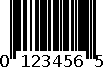
\includegraphics{../graphics/upceEg.pdf}
\]
%\begin{center}
%\begin{pspicture}(1.5,1.2in)
%\psbarcode{0123456}{includetext}{upce}
%\end{pspicture}
%\end{center}
These are compressed UPC-A codes where $5$ zeros have been
removed. The rules for transforming UPC-A codes to UPC-E codes are a
bit tedious, so we'll skip them for now---though they are easy
to look up on the internet.


\begin{question}
Can you find a UPC-E code and verify that it is valid?
\end{question}
\QM





\newpage

\subsection*{Problems for Section \thesection}\hrule\vspace{1ex}
\begin{enumerate}

\item Which of the following is a correct UPC-A number?% telescope 
\begin{align*}
&8\quad12556\;01041\quad0\\
&8\quad12565\;01091\quad0\\
&8\quad12556\;01091\quad0
\end{align*}
Explain your reasoning.


\item  Which of the following is a correct UPC-A number?% telescope 
\begin{align*}
&7\quad17664\;13387\quad0\\
&7\quad17669\;13387\quad0\\
&7\quad17669\;73387\quad0
\end{align*}
Explain your reasoning.


\item Find the missing digit in the following UPC-A number:
\[
8\quad14371\;0\blacksquare354\quad2
\]
Explain your reasoning.

\item Find the missing digit in the following UPC-A number:
\[
0\quad76484\;86\blacksquare97\quad3
\]
Explain your reasoning.

\item How similar can two different UPC numbers be? Explain your
  reasoning.
\item In the United States some bank check codes are nine digit
  numbers
\[
a_1 a_2 a_3 a_4 a_5 a_6 a_7 a_8 a_9
\] 
where
\[
7a_1 + 3a_2 + 9a_3 + 7a_4 + 3a_5 + 9a_6 + 7 a_7 + 3a_8 \equiv a_9 \pmod{10}.
\]
\begin{enumerate}
\item Give three examples of valid bank check codes.
\item If adjacent digits were accidentally switched, could a machine
  detect the error? Explain your reasoning.
\end{enumerate}
\item ISBN-10 numbers are ten digit
  numbers
\[
a_1 a_2 a_3 a_4 a_5 a_6 a_7 a_8 a_9 a_{10}
\] 
where
\[
10a_1 + 9a_2 + 8a_3 + 7a_4 + 6a_5 + 5a_6 + 4a_7 + 3a_8 +2a_9+a_{10}\equiv 0 \pmod{11}.
\]
\begin{enumerate}
\item Give three examples of ISBN-10 numbers.
\item If adjacent digits were accidentally switched, could a machine
  detect the error? Explain your reasoning.
\end{enumerate}
\end{enumerate}

\newpage



\section{The Binomial Theorem}


\subsection{Varna-Sangita}

In ancient Indian texts we find a description of a type of music
called \textit{varna-sangita}.\index{varna-sangita} This is music made
from a variation of long and short syllables. When performing a
varna-sangita, one starts off with a given number of short syllables
and ends with the same number of long syllables. In between these
verses, every possible combination of long and short syllables is
supposed to occur. If $s$ represents a short syllable and $l$
represents a long syllable we might visualize this as:
\[
ssss  \xto{\text{every possible combination}} llll
\]

To check their work, the people of ancient India counted how many of
each combination appeared in a song. Suppose we started with $sss$ and
finished with $lll$. Our song should contain the following verses:
\[
sss,\qquad ssl,\qquad sls, \qquad lss, \qquad sll,\qquad lsl, \qquad lls,\qquad lll
\]
We can construct the following table to summarize what we have found:
\[
\begin{tabular}{|c|c|c|c|}\hline
$3$ $s$'s & $2$ $s$'s and $1$ $l$ & $1$ $s$ and $2$ $l$'s & $3$ $l$'s \\ \hline
1 & 3 & 3 & 1\\\hline
\end{tabular}
\]

\begin{question} 
What would your table look like if you started with $ss$ and finished
with $ll$? What about if you started with $ssss$ and finished with
$llll$?
\end{question}
\QM

The vedics of the time gave a rule for making tables like the one
above. Their rule was based on the following diagram:
\[
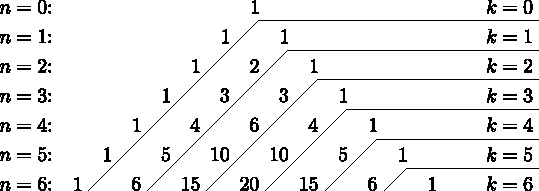
\includegraphics[scale=1]{../graphics/pascalsTri.pdf}
\]
Today people call this diagram \textbf{Pascal's
  triangle}.\index{Pascal's!triangle}
%\large %% Code used to help inkscape
%\[
%\begin{tabular}{rc@{}c@{}c@{}c@{}c@{}c@{}c@{}c@{}c@{}c@{}c@{}c@{}c@{}}
%$n=0$:&    &    &   &    &    &    &  1\\
%$n=1$:&    &    &   &    &    &  1 &    &  1\\
%$n=2$:&    &    &   &    &  1 &    &  2 &    &  1\\
%$n=3$:&    &    &   &  1 &    &  3 &    &  3 &    &  1\\
%$n=4$:&    &    & 1 &    &  4 &    &  6 &    &  4 &    &  1\\
%$n=5$:&    &  1 &    &  5 &    &  10 &    &  10 &    &  5 & & 1\\
%$n=6$:&  1 &    &  6 &    &  15 &    &  20 &    &  15 & & 6 & & 1\\
%\end{tabular}
%\]
%\[
%\begin{tabular}{r}
%$k=0$\\
%$k=1$\\
%$k=2$\\
%$k=3$\\
%$k=4$\\
%$k=5$\\
%$k=6$\\
%\end{tabular}
%\]

\begin{question}
How does Pascal's triangle relate to varna-sangitas? Is there an easy
way to produce the above diagram?
\end{question}
\QM

And now for something completely different\dots 

\subsection{Expansions}

Expand the following on a separate sheet of paper. Write the result
of your work in the boxes below:
\begin{align*}
(a + b)^0 &=  \raisebox{-3mm}{\fbox{\rule[0mm]{0mm}{7mm}\hspace{50ex}}} \\
(a + b)^1 &=  \raisebox{-3mm}{\fbox{\rule[0mm]{0mm}{7mm}\hspace{50ex}}} \\
(a + b)^2 &=  \raisebox{-3mm}{\fbox{\rule[0mm]{0mm}{7mm}\hspace{50ex}}} \\
(a + b)^3 &=  \raisebox{-3mm}{\fbox{\rule[0mm]{0mm}{7mm}\hspace{50ex}}} \\
(a + b)^4 &=  \raisebox{-3mm}{\fbox{\rule[0mm]{0mm}{7mm}\hspace{50ex}}} 
\end{align*}

\begin{question} Is there a nice way to organize this data?
\end{question}
\QM

\begin{question}
Can you explain the connection between expanding binomials and
varna-sangitas?
\end{question}
\QM

\begin{activitynote}
Activity~\ref{A:traffic} complements this section well.  % On the Road
\end{activitynote}



\subsection{Come Together}

Let's see if we can bring these ideas together. Let's denote the following symbol:
\[
\binom{n}{k} = \text{the number of ways we choose $k$ objects from $n$
  objects}.\index{nchoosek@$\binom{n}{k}$}\index{nck@$_nC_k$}
\]
it is often said ``$n$ choose $k$'' and is sometimes denoted as $_n C_k$.

\begin{question}
What exactly does $\binom{n}{k}$ mean in terms of varna-sangitas? What
does $\binom{n}{k}$ mean in terms of expansion of binomials?
\end{question}
\QM

\begin{question} How does $\binom{n}{k}$ relate to Pascal's triangle?
\end{question}
\QM


\begin{question}
Pascal claims:
\[
\binom{n}{k-1} +  \binom{n}{k} = \binom{n+1}{k}
\]
Explain how this single equation basically encapsulates the key
to constructing Pascal's triangle.
\end{question}
\QM

\begin{question}
Suppose that an oracle tells you that
\[
\binom{n}{k} = \frac{n!}{k!(n-k)!}
\]
but we, being good skeptical people, are not convinced. How do we
check this?
\end{question}
\QM

From the work above, we obtain a fabulous theorem:


\begin{theorem}[Binomial Theorem]\index{Binomial Theorem} 
If $n$ is a nonnegative integer, then
\[
(a+b)^n = \binom{n}{0} a^nb^0 + \binom{n}{1} a^{n-1}b^1 + \dots + \binom{n}{n-1} a^{1}b^{n-1} + \binom{n}{n} a^{0}b^n.   
\]
\end{theorem}


\begin{question} 
This looks like gibberish to me. Tell me what it is saying. Also, why
is the Binomial Theorem true?
\end{question}
\QM



\begin{activitynote}
Activity \ref{A:factOrFiction} complements this section well.  % Pascal's Triangle: Fact or Fiction
\end{activitynote}


\begin{activitynote}
Activity~\ref{A:pyramid} is worth considering here.  % Pascal's Pyramid
\end{activitynote}


\begin{activitynote}
The counting/probability activities, \ref{A:countOnIt} through \ref{A:fallForAnything} can now be done.
% You Can Count on It
% Which Road Should We Take
% Lumpy and Eddie
% Go Climb a Tree
% They'll Fall for Anything
\end{activitynote}



\newpage
\begin{problems}
\begin{enumerate}
\item Write down the first $7$ rows of Pascal's triangle.
\item Explain how $\binom{n}{k}$ corresponds to the entries of Pascal's
  triangle. Feel free to draw diagrams and give examples.
\item State the Binomial Theorem and give some examples of it in action.
\item Explain the ``physical'' meaning of $\binom{n}{k}$. Give some
  examples illustrating this meaning.
\item\label{P:bfor} Explain how Pascal's triangle is formed. In your
  explanation, use the notation $\binom{n}{k}$. If you were so
  inclined to do so, could you state a single equation that basically
  encapsulates your explanation above?
\item Explain why the formula you found in Problem \ref{P:bfor} is
  true.
\item State the formula for $\binom{n}{k}$.
\item Expand $(a + b)^5$ using the Binomial Theorem.
\item Expand $(a - b)^7$ using the Binomial Theorem.
\item Expand $(-a - b)^8$ using the Binomial Theorem.
\item Expand $(a + (b + c))^3$ using the Binomial Theorem.
\item Expand $(a - b - c)^3$ using the Binomial Theorem.
\item\label{P:exp1} Let $n$ be a positive integer.
\begin{enumerate}
\item Try some experiments to guess when $9^n + 1^n$ is
  divisible by $10$. What do you find? Clearly articulate your
  conjecture.
\item Use the Binomial Theorem to explain why your conjecture is
  true. Hint: $10-9 = 1$.
\end{enumerate}
\item\label{P:exp2} Let $n$ be a positive integer.
\begin{enumerate}
\item Try some experiments to guess when $6^n + 4^n$ is divisible by
  $10$. What do you find? Clearly articulate your conjecture.
\item Use the Binomial Theorem to explain why your conjecture is
  true. Hint: $10-6 = 4$.
\end{enumerate}
\item\label{P:exp3} Let $n$ be a positive integer.
\begin{enumerate}
\item Try some experiments to guess when $7^n - 3^n$ is divisible by
  $10$. What do you find? Clearly articulate your conjecture.
\item Use the Binomial Theorem to explain why your conjecture is
  true. Hint: $10-3 = 7$.
\end{enumerate}
\item\label{P:exp4} Let $n$ be a positive integer.
\begin{enumerate}
\item Try some experiments to guess when $8^n - 2^n$ is divisible by
  $10$. What do you find? Clearly articulate your conjecture.
\item Use the Binomial Theorem to explain why your conjecture is
  true. Hint: $10-2 = 8$.
\end{enumerate}
\item Generalize Problems \ref{P:exp1}, \ref{P:exp2}, \ref{P:exp3},
  and \ref{P:exp4} above. Clearly articulate your new statement(s) and
  explain why they are true.
\item\label{P:e1} Which is larger, $(1 + 1/2)^2$ or $2$? Explain your
  reasoning.
\item\label{P:e2} Which is larger, $(1 + 1/5)^5$ or $2$? Explain your
  reasoning.
\item\label{P:e3} Which is larger, $(1 + 1/27)^{27}$ or $2$? Explain
  your reasoning.
\item\label{P:e4} Which is larger, $(1 + 1/101)^{101}$ or $2$? Explain
  your reasoning.
\item\label{P:e5} Which is larger, $(1.0001)^{10000}$ or $2$? Explain
  your reasoning.
\item Generalize Problems \ref{P:e1}, \ref{P:e2}, \ref{P:e3},
  \ref{P:e4}, and \ref{P:e5} above. Clearly articulate your new
  statement(s) and explain why it is true.
\item Given a positive integer $n$, can you guess an upper bound for
  $(1 + 1/n)^{n}$?
\item Let $n$ be a positive integer. Use the Binomial Theorem to
  explain why:
\[
\binom{n}{0} + \binom{n}{1} + \binom{n}{2} + \dots + \binom{n}{n} = 2^n
\]
What does this mean in terms of Pascal's Triangle?
\item Let $n$ be a positive integer. Use the Binomial Theorem to
  explain why:
\[
(-1)^0\binom{n}{0} + (-1)^1\binom{n}{1} + (-1)^2\binom{n}{2} + \dots + (-1)^n\binom{n}{n} = 0
\]
What does this mean in terms of Pascal's Triangle?
\item Suppose I tell you:
\[
(1+x)^n = \binom{n}{0} + \binom{n}{1}x + \binom{n}{2}x^2+\dots +
\binom{n}{n}x^n
\]
Explain how to deduce:
\[
(a+b)^n = \binom{n}{0}a^n + \binom{n}{1}a^{n-1}b +
\binom{n}{2}a^{n-2}b^2+\dots + \binom{n}{n}b^n
\]
\end{enumerate}
\end{problems}



